\documentclass[a4paper,12pt]{article}

\usepackage[utf8]{inputenc}
\usepackage[T2A]{fontenc} 
\usepackage[serbianc]{babel}
\usepackage{graphicx}
\usepackage{wrapfig}
\usepackage{xcolor}
\usepackage{amsmath}
\usepackage{amsthm}
\usepackage{hyperref}

\newtheorem{teorema}{Теорема}
\newtheorem{definicija}{Дефиниција}

\title{Друмски тркачки мотоцикли}
\author{Филип Петровић, 255/2025}
\date{\today}

\begin{document}

\maketitle
\tableofcontents
\newpage

\section{Увод}
Тркачки мотоцикли су машине високих перформанси направљене за рад при великим брзинама и са одличном контролом на асфалтираним стазама, од модификованих уличних мотоцикала (Суперсток) до прототипова направљених по мери (МотоГП). Кључне карактеристике су аеродинамични оклопи, агресиван положаје вожње, снажан агрегат и напредне кочнице. С обзиром да се возе само по тркачким стазама, нису им неопходна светала и ретровизори, па се они скидају ради безбедности и смањења тежине. Ови мотоцикли се такмиче у класама као што су МотоГП, Супербајк (модификовани производни мотоцикли) и Суперсток, захтевајући прецизност и техничке вештине од возача.

\section{Динамика кретања}

\begin{wrapfigure}{l}{0.4\textwidth}
    \centering
    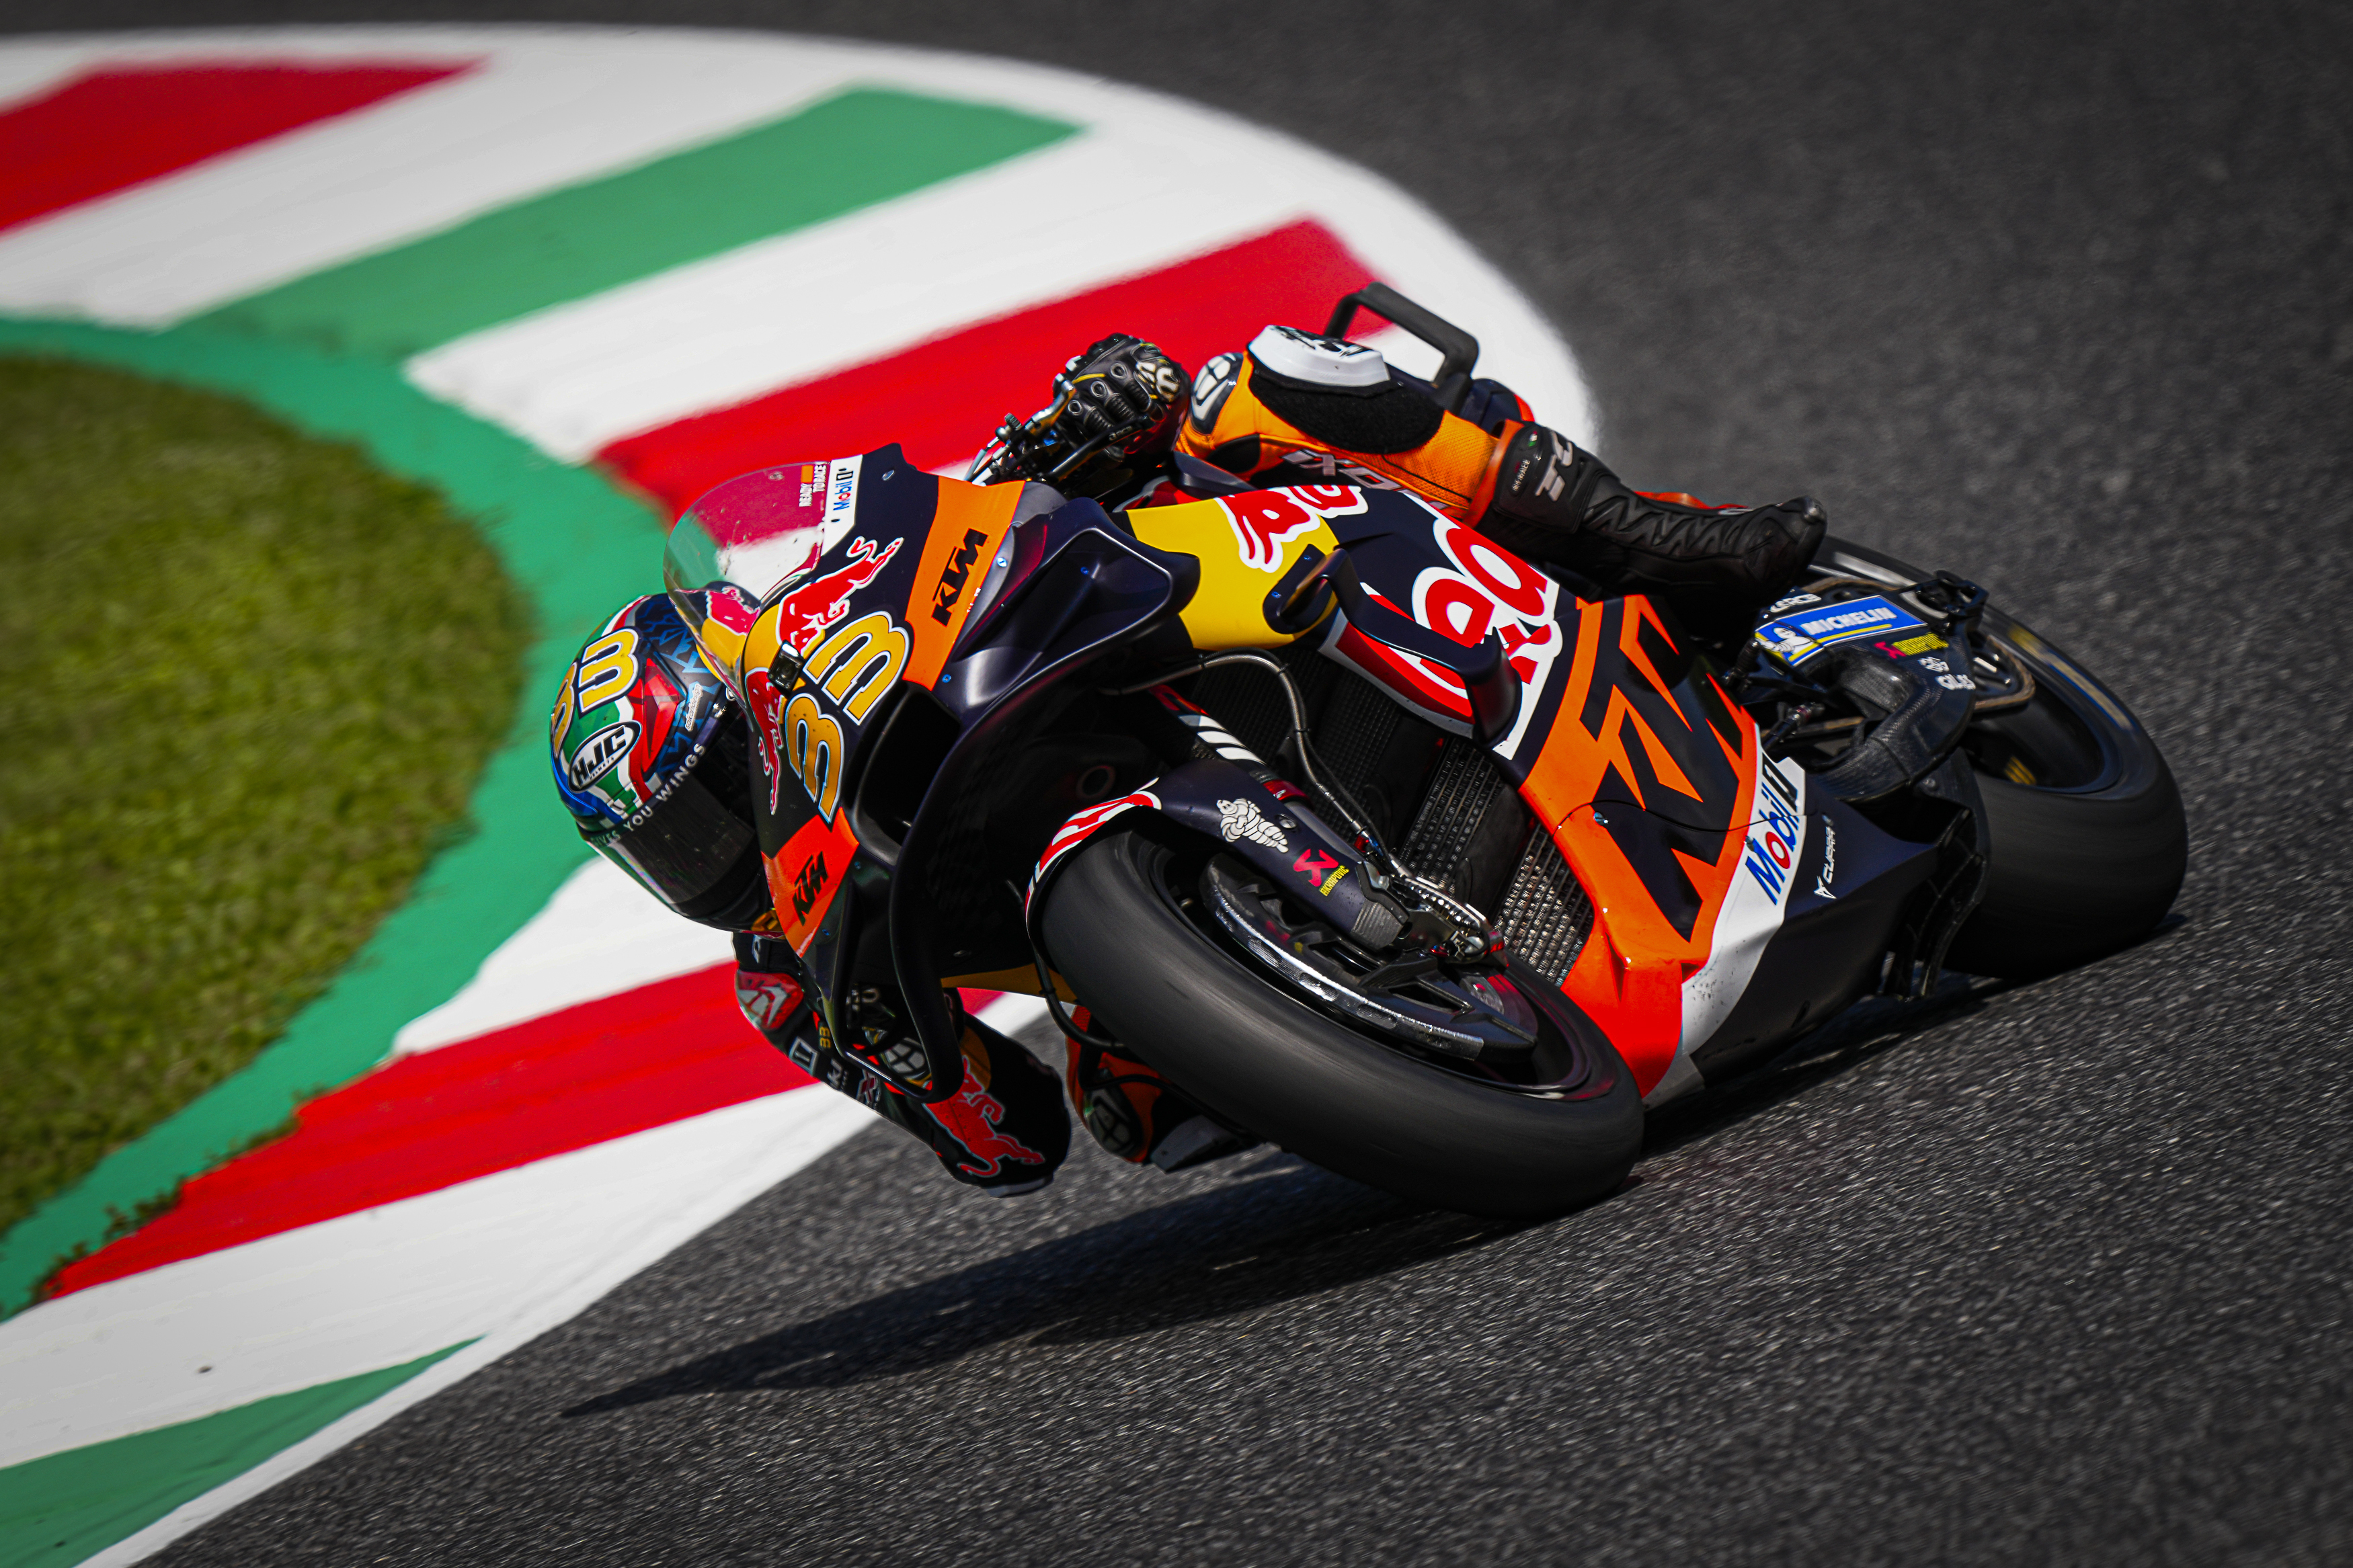
\includegraphics[width=0.35\textwidth]{slike/motor2.jpg}
    \caption{Мотоцикл у кривини}
\end{wrapfigure}

Нагињање мотоцикла је неопходно за скретање, неопходно је доводести у равнотежу центрифугалну силу коју мотор прави и гравитациону силу над тежиштем мотора. Техника се покреће кратким, супротним притиском на управљач (coutersteering) чиме се мотор избацује из равнотеже и креће да скреће у правцу у којем га возач усмерава. Правилна техника укључује померање телесне тежине, опуштање руку и притискање унутрашњег управљача како би се смањио угао нагиба мотоцикла. Угао нагиба често прелази \textcolor{red}{60 степени}. 

\subsection{Математички модел}
Кинетичка енергија мотоцикла при максималној брзини се рачуна по формули:

$$ E_k = \frac{1}{2} m v^2 $$

Где је $m$ маса система (мотор + возач), а $v$ брзина кретања.

\section{Теоријске основе}

\begin{definicija}
\textbf{Траг кочења} је растојање које мотоцикл пређе од тренутка активирања кочнице до потпуног заустављања.
\end{definicija}

\begin{teorema}
Стабилност мотоцикла при великим брзинама директно је пропорционална жироскопском ефекту точкова.
\end{teorema}

\section{Компоненте и нјихове цене}

Цене неких од компоненти МотоГП мотоцикла:

\begin{table}[h]
\centering
\begin{tabular}{|l|c|r|}
\hline
\textbf{Компонента}  & \textbf{Цена (\$)} \\
\hline
Агрегат & 600.000
Карбонски рам и оклоп & 300.000 \\
Мењач & 150.000 \\
ЕЦУ & 100.000 \\
Вешање & 80.000 \\
Кочнице & 50.000 \\
Ауспух & 10.000 \\
\hline
\end{tabular}
\caption{Цене компонената MotoGP машине}
\end{table}

\section{Закључак}
Иако на први поглед делује да трке мотора (конкретно МотоГП) доприносе само забави гледаоца, доста технологија које су развијене за тркачке мотоцикле се касније нађу на обичним мотоциклима, тако да развој тркачких мотоцикала доприноси унапређењу технологији и безбедности у друмском саобраћају.

\end{document}